\section{Logik}
\textcolor{myblue}{Nulläre Funktion:} Funktion mit null Parametern\\
Bsp.: $f() = 1$ \quad		=> eine Möglichkeit mit null Argumenten\\
\textcolor{myblue}{Unäre Funktion:} Funktion mit einem Parameter\\
Bsp.: $f(x) --> x$ \quad	=> Zwei mögliche Argumente: x=0 oder x=1\\
\textcolor{myblue}{Binäre Funktion:} Funktion mit zwei Parametern\\
Bsp.: $f(x, y) = x \wedge y$ \quad	=> 4 mögl. Argumente (0,0),(0,1),(1,0),(1,1)\\
\textcolor{myblue}{n-äre Funktion:} Funktion mit n Parametern (n-stellig)\\
Bsp: $f (x_0,...,x_{n-1}) = x_0 \wedge x_1 \wedge ... \wedge x_{n-1} \Rightarrow 2^n$ mögliche Kombinationen
\subsection{Disjunktion \& Konjunktion}
Neutrales Element:
\vspace{-0.32cm}
\begin{multicols*}{2}
$(x \vee 0) \equiv (x)$\\ 
$(x \wedge 1) \equiv (x)$\\
\end{multicols*}
\vspace{-0.50cm}

Komplement:
\vspace{-0.32cm}
\begin{multicols*}{2}
$(x \vee \neg x) \equiv (1)$\\ 
$(x \wedge \neg x) \equiv (0)$\\ 
\end{multicols*}
\vspace{-0.50cm}

Kommutativität:
\vspace{-0.32cm}
\begin{multicols*}{2}
$(x \wedge y) \equiv (y \wedge x)$\\ 
$(x \vee y) \equiv (y \vee x)$\\
\end{multicols*}
\vspace{-0.50cm}

Assoziativität:
\vspace{-0.32cm}
\begin{multicols*}{2}
$(x \wedge (y \wedge z)) \equiv ((x \wedge y) \wedge z)$\\
$(x \vee (y \vee z)) \equiv ((x \vee y) \vee z)$\\
\end{multicols*}
\vspace{-0.50cm}

Distributivität:
\vspace{-0.32cm}
\begin{multicols*}{2}
$(x \wedge (y \vee z)) \equiv ((x \wedge y) \vee (x \wedge z))$\\
$(x \vee (y \wedge z)) \equiv ((x \vee y) \wedge (x \vee z))$\\
\end{multicols*}
\vspace{-0.50cm}

Idempotenz:
\vspace{-0.32cm}
\begin{multicols*}{2}
$(x \wedge x) \equiv x$\\
$(x \vee x) \equiv x$\\
\end{multicols*}
\vspace{-0.50cm}

Doppelnegation:
$\neg (\neg x) \equiv x$

de Morgans Regeln:
\vspace{-0.32cm}
\begin{multicols*}{2}
$\neg (x \wedge y) \equiv ((\neg x) \vee (\neg y))$\\
$\neg (x \vee y) \equiv ((\neg x) \wedge (\neg y))$\\
\end{multicols*}
\vspace{-0.50cm}

\subsection{Exklusive Disjunktion (XOR) }
Abbildung der Addition zweier Bits und die Konjunktion den Übertrag.

\subsection{16 Binäre Funktionen}
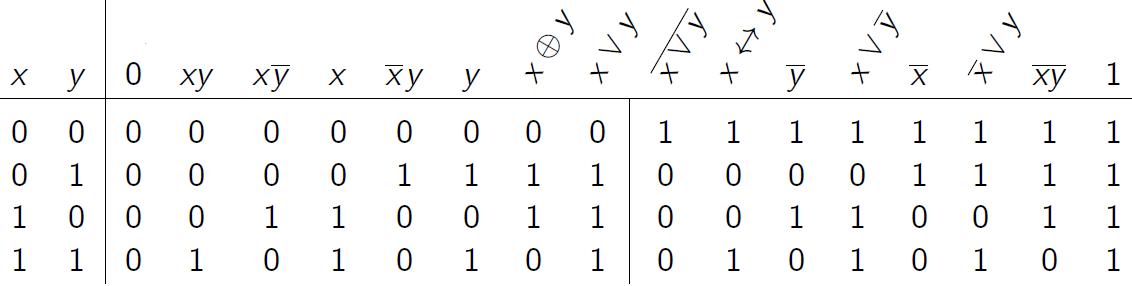
\includegraphics[width=\columnwidth]{binary_functions}
2 nulläre: $0, 1$ \quad 4 unäre: $x, y, \neg x, \neg y$